\section{Architecture and Implementation}


The architecture of the Safety Annex is shown in Figure~\ref{fig:plugin-arch}.  It is written in Java as a plug-in for the OSATE AADL toolset, which is built on Eclipse.  It is not designed as a stand-alone extension of the language, but works with behavioral contracts specified AGREE AADL annex and associated tools~\cite{NFM2012:CoGaMiWhLaLu}.  AGREE allows {\em assume-guarantee} behavioral contracts to be added to AADL components.  The language used for contract specification is based on the Lustre dataflow language~\cite{Halbwachs91:IEEE}. AGREE improves scalability of formal verification to large systems by decomposing the analysis of a complex system architecture into a collection of smaller verification tasks that correspond to the structure of the architecture.

\begin{figure}
\begin{center}
%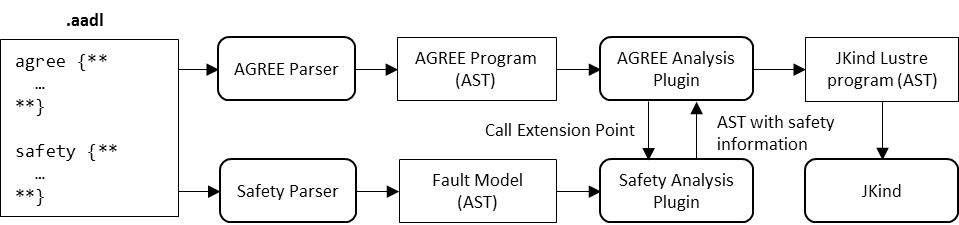
\includegraphics[trim=0 400 430 0,clip,width=0.85\textwidth]{images/arch.png}
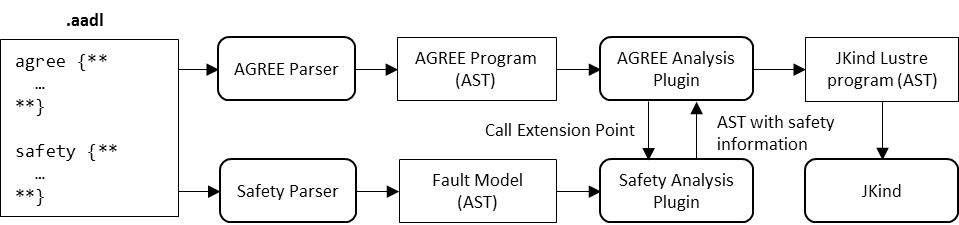
\includegraphics[width=.9\textwidth]{images/arch.png}
\end{center}
\vspace{-0.2in}
\caption{Safety Annex Plug-in Architecture}
\label{fig:plugin-arch}
\end{figure}

AGREE contracts are used to define the nominal behaviors of system components as {\em guarantees} that hold when {\em assumptions} about the values the component's environment are met.  The Safety Annex extends these contracts to allow faults to modify the behavior of component inputs and outputs.  To support these extensions, AGREE implements an Eclipse extension point interface that allows other plug-ins to modify the generated abstract syntax tree (AST) prior to its submission to the solver.  If the Safety Annex is enabled, these faults are added to the AGREE contract and, when triggered, override the nominal guarantees provided by the component.  An example of a portion of an initial AGREE node and its extended contract is shown in Figure~\ref{fig:comp}.  The \texttt{\_\_fault} variables and declarations are added to allow the contract to override the nominal behavioral constraints (provided by guarantees) on outputs.  In the Lustre language, \texttt{assertion}s are constraints that are assumed to hold in the transition system.

\begin{figure}
\vspace{-0.1in}
%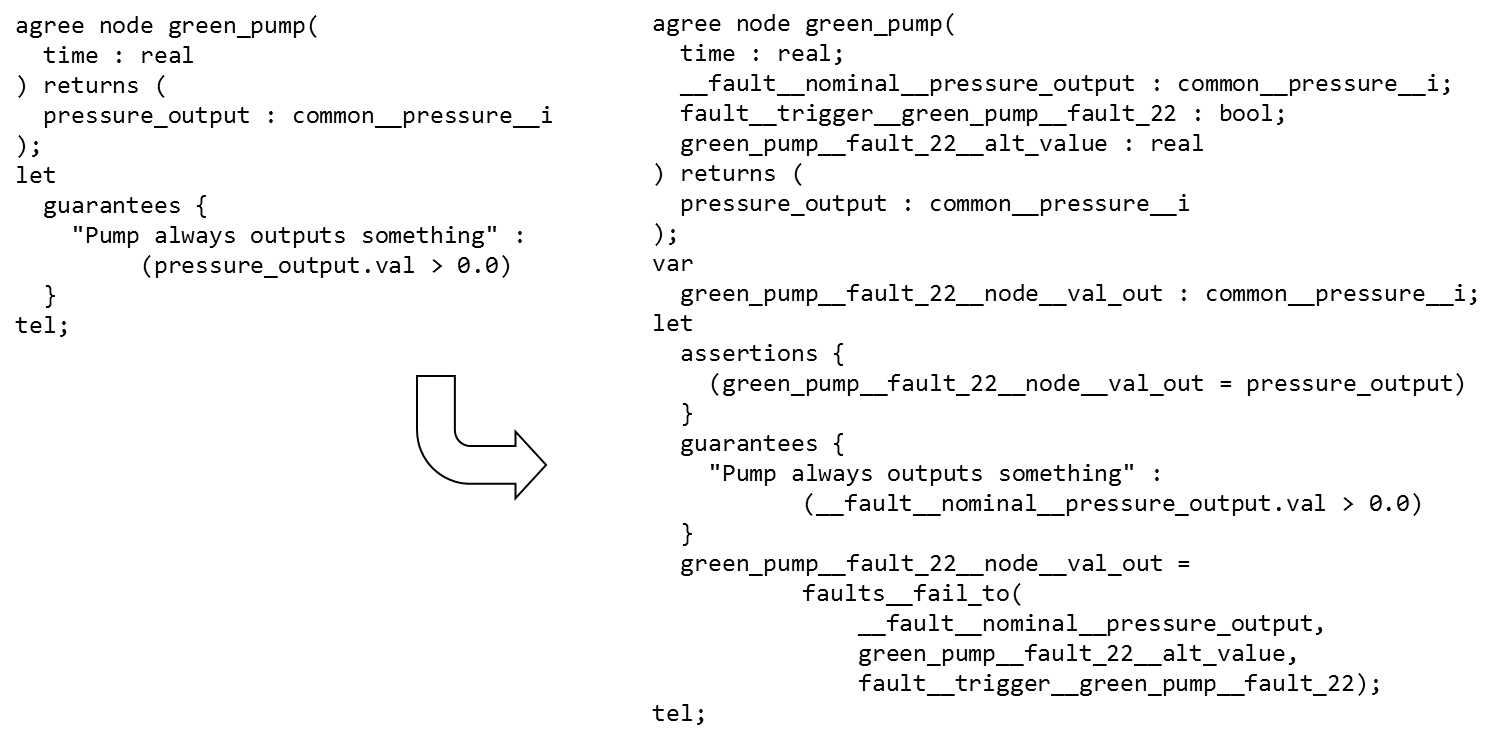
\includegraphics[trim=30 150 120 10,clip,width=\textwidth]{images/sample_code.png}
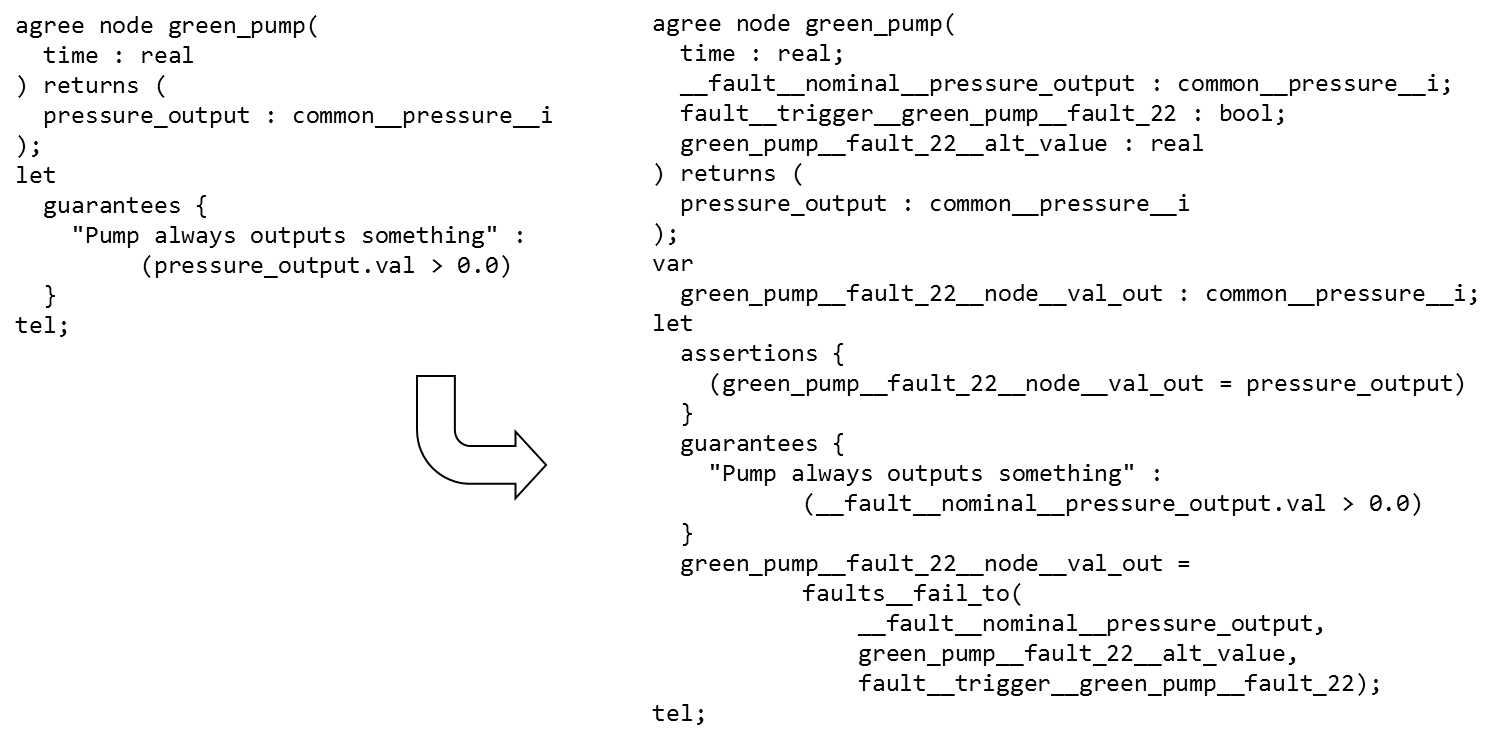
\includegraphics[width=\textwidth]{images/sample_code.png}
\vspace{-0.3in}
\caption{Nominal AGREE node and its extension with faults}
\label{fig:comp}
\end{figure}

An annotation in the AADL model determines the fault hypothesis.  This may specify either a maximum number of faults that can be active at any point in execution (typically one or two), or that only faults whose probability of simultaneous occurrence is above some probability threshold should be considered.  In the former case, we assert that the sum of the true {\em fault\_\_trigger} variables is below some integer threshold.  In the latter, we determine all  combinations of faults whose probabilities are above the specified probability threshold, and describe this as a proposition over {\em fault\_\_trigger} variables.

Once augmented with fault information, the AGREE model follows the standard AGREE translation path to the model checker JKind~\cite{2017arXiv171201222G}, an infinite-state model checker for safety properties.  The augmentation includes traceability information so that when counterexamples are displayed to users, the active faults for each component are visualized.



